% See author's guidelines for Methods in Ecology and Evolution:
% http://www.methodsinecologyandevolution.org/view/0/authorGuidelines.html

\documentclass[12pt]{article}

% One-inch margins
\usepackage{fullpage}

% No orphans or widows
\usepackage[all]{nowidow}

% Additional math features
\usepackage{amsmath}

% Use mee bibliography style
\usepackage{natbib}
\bibliographystyle{mee}

% Include figures
\usepackage{graphicx}

% Definitions to make it easier to type
\newcommand{\MCMCMC}{(MC)$^{3}$}
\newcommand{\MCMCMCMC}{(MC)$^{4}$}

\begin{document}

% Double-spaced
\baselineskip 24pt

\begin{flushleft}

{\Large\textbf{Identifying rate shifts on phylogenetic trees using BAMM
    with multi-core Metropolis coupled Markov chain Monte Carlo}}

% Short title must be <= 45 characters (current: 44, including spaces)
\textbf{Short title:} BAMM with multi-core Metropolis coupled MCMC

% Recommended: 6000-7000 words, including tables, figure captions, references
\textbf{Word count:} 3,218

Carlos J. R. Anderson$^{1}$ and
Daniel L. Rabosky$^{1,*}$

$^{1}$Department of Ecology and Evolutionary Biology,
    University of Michigan, Ann Arbor, MI 48109, USA

$^{*}$Corresponding author: Daniel L. Rabosky (drabosky@umich.edu)

\end{flushleft}


\pagebreak[4]


% Maximum of 350 words
\section*{Abstract}

% Suppress indentation for the following paragraphs
{\setlength{\parindent}{0cm}

\textbf{1.}
BAMM (Bayesian Analysis of Macroevolutionary Mixtures) is a computer program
that uses reversible jump Markov chain Monte Carlo (rjMCMC)
to model complex dynamics of speciation, extinction,
and trait evolution on phylogenetic trees.
%
Previous versions of BAMM used a single Markov chain
to explore the landscape of models and their parameter values.
%
A single chain, however, may get stuck in local optima,
resulting in poor performance in both mixing and convergence.

\textbf{2.}
Here we describe an extension to BAMM
that implements Metropolis coupled MCMC [\MCMCMC].
%
With \MCMCMC, additional chains are introduced
that are able to explore more of the model landscape.
%
Swaps between chains may occur periodically,
so if a chain is stuck in a local optimum,
it may immediately jump to another area of the landscape.
%
In addition, we describe multi-core \MCMCMC\ [\MCMCMCMC]
which runs each chain on a separate computer processor.

\textbf{3.}
Using both simulated phylogenetic trees and an empirical tree,
we find that runs with \MCMCMC\ mix better than those with a single chain.
%
In simulated trees, convergence in runs with or without \MCMCMC\ 
is about the same, but in an empirical example tree,
convergence is better in runs with \MCMCMC\ than those without.
%
\MCMCMCMC\ speeds up run times by a factor of approximately $n$
in runs with $n$ chains.

\textbf{4.}
\MCMCMC\ and \MCMCMCMC\ greatly improve
the efficiency and speed of runs in BAMM,
and we recommend their use in future studies of macroevolutionary dynamics.
}

\begin{flushleft}
\textbf{Key-words:} BAMM, Bayesian, macroevolution, phylogeny, diversification, speciation
\end{flushleft}


\pagebreak[4]


% State the reason for the work, the context and the hypotheses being tested
\section*{Introduction}

\subsection*{Background}

The variation in species richness and phenotypic diversity we see today
across groups of organisms is partly due to the stochastic
evolutionary processes of speciation and extinction \citep{rab14plos}.
%
Rates of speciation, extinction, and phenotypic evolution
have changed through time and among groups
as a result of unique historical events,
such as environmental, phenotypic, and genetic changes.
%
For example, speciation could dramatically increase
during adaptive radiation on a newly colonized island \citep{sch00,los10}.
%
Potentially, phenotypic evolutionary rates for this colonizing group
might also increase as organisms adapt and fill
available ecological niches \citep{mah10}.
%
Speciation rates might increase following the evolution of key traits
that facilitate novel patterns of resource use \citep{mit88}
or which increase the rate at which isolated lineages
evolve reproductive isolation \citep{pan01,coy04}.


The processes of speciation and extinction are expected to leave a signal
in the topology and branch lengths of phylogenetic trees (Nee et al. 1994).
%
Phylogenies can thereferore be used to extract information
about the evolutionary processes that shaped them.
%
With an appropriate phylogenetic framework,
distributions of phenotypic traits across phylogenies
can provide information about the tempo and mode of morphological evolution
(citations...).
%
A major challenge in phylogenetic diversification studies
(speciation, extinction, or trait evolution)
has been to accommodate the complex mixture of dynamics
that have shaped real phylogenetic trees and trait distributions \citep{ome12}.
%
As researchers generate ever-larger phylogenies
\citep{jet12,pyr13,rab13,zan14}, it is increasingly important
to account for the possibility that evolutionary rates have been non-uniform,
both through time and among lineages.
%
A number of frameworks have recently been developed
that aim to account for heterogeneous evolutionary processes
across phylogenetic trees \citep{rev12,eas11,alf09,ven11,tho12}.
%
We recently developed a new method to identify and characterize
complex mixtures of heterogeneous macroevolutionary dynamics
across phylogenetic trees \citep{rab14plos,rab13}.


\subsection*{BAMM and Markov chain Monte Carlo}

BAMM (Bayesian Analysis of Macroevolutionary Mixtures)
is a computer program that characterizes complex processes of
diversification (i.e., speciation and extinction)
or phenotypic evolution on phylogenetic trees.
%
BAMM assumes that trees are shaped by heterogeneous mixtures
of distinct evolutionary rate regimes.
%
Each distinct evolutionary rate regime is modeled as a time-varying or
time-constant rate process. For example, speciation rates can
be modeled using a time-dependent exponential change function.
%
We describe the tree as a heterogeneous collection of
such processes, because processes
are independent---each one has its own parameter values.
%
Thus, one process may indicate an increase in speciation rate,
while another may indicate a decrease in speciation rate
within the same tree (Figure~\ref{fig:tree}).

\begin{figure}
\begin{center}
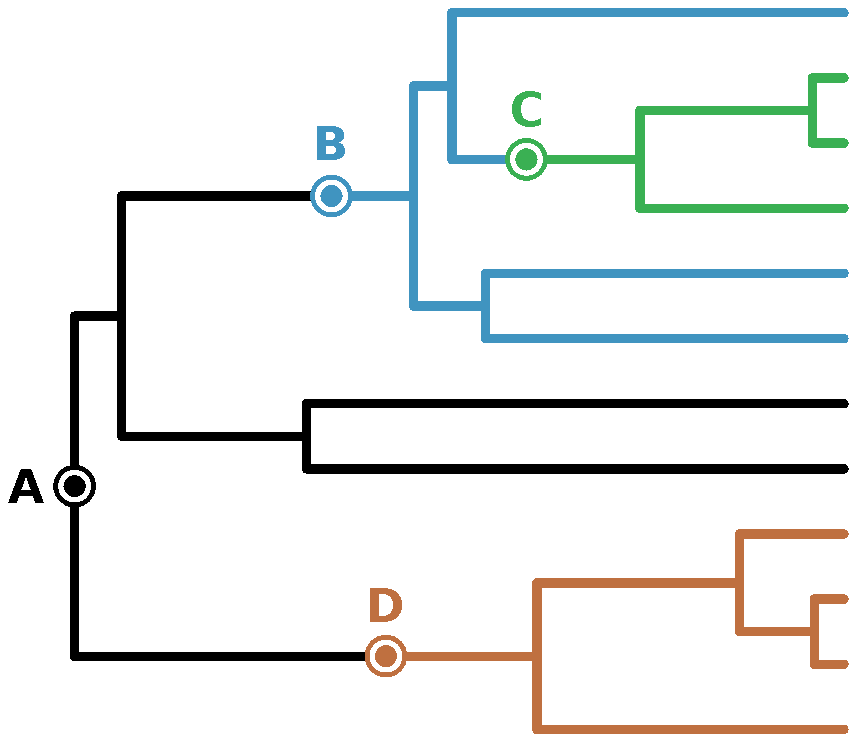
\includegraphics[width=7cm]{tree.pdf}
\end{center}
\caption{Phylogenetic tree with a mixture of macroevolutionary processes.
    Each colored circle (A--D) is an event,
    which marks the start of a new process.
    Branches that share the same color share the same process.
    The root event (A) marks the start of the background process,
    and events B--D represent shifts to different processes.}
\label{fig:tree}
\end{figure}


We call the start of a process an \emph{event} or \emph{shift},
which may occur on any branch of the tree
(e.g., colored circles in Figure~\ref{fig:tree}).
%
The number of events on a tree follow a compound Poisson process.
%
All branches downstream of an event share the same process
(e.g., all branches downstream of event D
in Figure~\ref{fig:tree} share the same process).
%
An event may occur within a clade controlled by another process.
(e.g., event C in Figure~\ref{fig:tree}).
%
In such a case, the process downstream of the \emph{ancestral} process
takes over the dynamics of the branches downstream of it.
%
A tree must always have a process at its root.
(e.g., event A in Figure~\ref{fig:tree}).


BAMM uses reversible jump Markov Chain Monte Carlo (rjMCMC) \citep{gre95}
to sample macroevolutionary rate shift configurations in proportion to their
posterior probability \citep{rab14plos}.
%
In BAMM, rjMCMC works by proposing changes, or \emph{moves},
to the current shift configuration
(e.g., adding or deleting an event,
moving the location of an event,
and changing specific parameter values of an event).
%
If the move improves the posterior probability of the new configuration,
the move is accepted and the new configuration becomes the current one.
%
Otherwise, the move is accepted with a probability proportional
to the ratio of probabilities of the proposed and current configurations.


If the move does not change the dimensionality of the shift configuration
(i.e., adding or deleting events),
the acceptance probability follows the Metropolis-Hastings formula:
\[\alpha = \text{min}\left\{ 1,
    \frac{f(\theta')}{f(\theta)} \times
    \frac{\pi(\theta')}{\pi(\theta)} \times
    \frac{q(\theta | \theta')}{q(\theta' | \theta)}
\right\}\]
where $\theta$ and $\theta'$ are parameter vectors
corresponding to the current and proposed states,
$f$ and $\pi$ are the corresponding likelihood and prior density functions,
and $q(\theta' | \theta)$ is the relative probability
of proposing a move to parameter vector $\theta'$,
given that the current state is $\theta$.
%
For moves that change the dimensionality---%
where reversible jump becomes important---%
a more general equation is used \citep[see][]{rab14plos,gre95}.


At the end of the MCMC simulation,
one obtains a set of configurations that are, theoretically,
a sample from the true posterior probability distribution
of macroevolutionary rate shift configurations.
%
A particular mapping of distinct evolutionary rate regimes
across a phylogenetic tree \citep{rab14sysbio,rab14mee}
is expected to be sampled in proportion to its posterior probability.
%
The advantage of using MCMC
is that BAMM does not produce a single best configuration,
but rather a set of configurations and their probability
of explaining the shape or data of the tree \citep{rab14plos}.
%
Therefore, if multiple shift configurations
explain the phylogenetic data similarly well,
they will be sampled at about the same frequency.


\subsection*{Metropolis coupled MCMC}

BAMM was originally implemented using a single Markov chain
to explore the landscape of model configurations and their parameter values.
%
A single chain, however, may get stuck in local optima,
resulting in less mixing and more time needed for convergence \citep{alt04}.
%
Mixing refers to how independent the samples are in a chain,
and convergence refers to how well the chain
approximates the true posterior distribution \citep{giv05}.
%
Here we describe an extension to BAMM
that implements Metropolis coupled MCMC [\MCMCMC].
%
In \MCMCMC, additional chains are introduced
that are able to explore more of the model landscape.
%
These additional chains are \emph{heated},
which means that the probability landscape is flattened
and therefore are able to explore more of it
and are less likely to get stuck.
%
Swaps between chains may occur periodically,
so if a chain does get stuck in a local optimum,
it may immediately jump to another area of the landscape
(Figure~\ref{fig:mc3-swap}).
%
To offset the computational cost of \MCMCMC, we implement
multi-core \MCMCMC\ [\MCMCMCMC], where each chain
runs on a separate computer processer in parallel to other chains,
decreasing the total amount of time the run would otherwise take.

\begin{figure}
\begin{center}
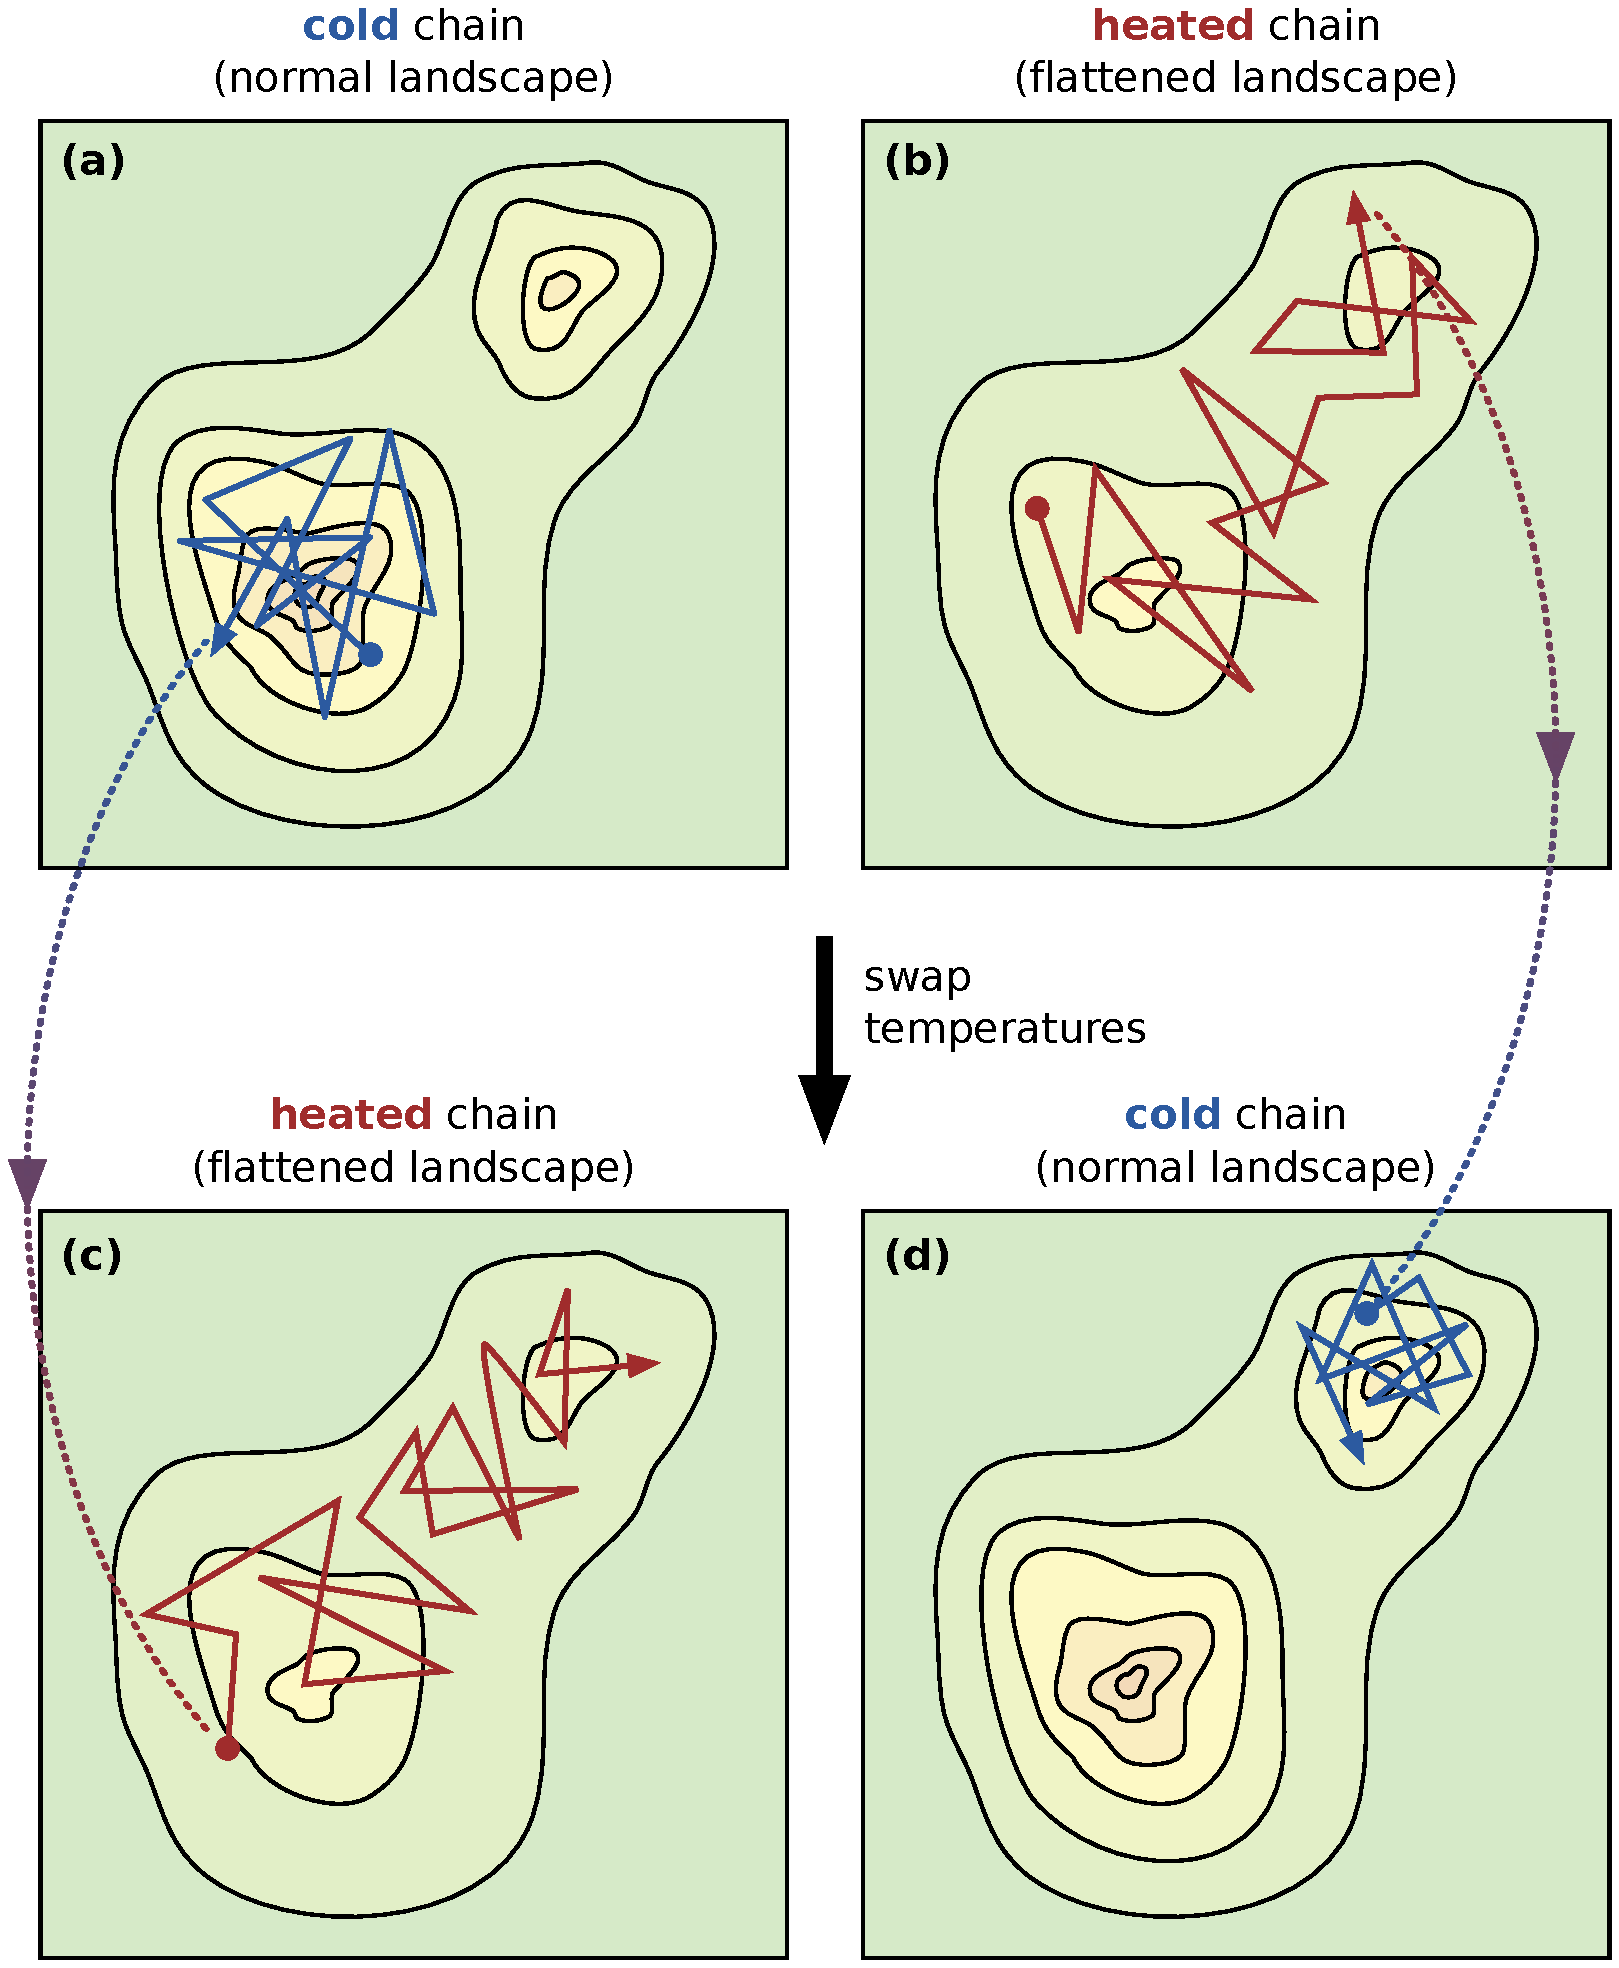
\includegraphics[width=11cm]{mc3-swap.pdf}
\end{center}
\caption{In Metropolis-coupled MCMC, the cold chain (a)
    is the chain whose samples are recorded, and it explores
    the same probability landscape as a regular MCMC.
    The heated chain (b) explores a flatter landscape.
    Heated chains (there may be more than one) are therefore
    able to cross valleys more effectively than the cold chain.
    After a certain number of generations,
    a swap in temperatures may occur between chains.
    The cold chain becomes heated (c) and the heated chain
    becomes the cold chain (d).
    A swap causes the cold chain to sample from
    where the heated chain left off (arrow from b to d).
    Thus, if the previous cold chain had been stuck in one area (a)
    a swap helps the cold chain get unstuck by jumping
    to a different area of the landscape (d).}
\label{fig:mc3-swap}
\end{figure}


% Include sufficient details for the work to be repeated
\section*{Materials and methods}

\subsection*{\MCMCMC\ and \MCMCMCMC\ implementation in BAMM}

We followed \citet{alt04} for the implementation of \MCMCMC\ in BAMM.
%
For each Markov chain $i \in \{1, 2, \dots\}$, its temperature was set to
$\beta_i = [1 + \Delta T \times (i - 1)]^{-1}$,
where $\Delta T$ is the temperature increment parameter.
%
For example, if there are 4 chains and $\Delta T$ is 0.1,
the temperature of each chain is 1, 0.9091, 0.8333, and 0.7692.
%
The cold chain always has a temperature of 1.
%
The value of $\Delta T$ should be greater than 0
and chosen such that the probability of accepting a swap
is between 20\% and 60\% \citep{alt04}.


The acceptance probability $\alpha_i$ for a move proposal in chain $i$
is a function of the temperature $\beta_i$.
%
For moves that do not involve changes in the dimensionality of the model,
\[\alpha_i = \text{min}\left\{ 1,
    \left(
    \frac{f(\theta_i')}{f(\theta_i)} \times
    \frac{\pi(\theta_i')}{\pi(\theta_i)}
    \right)^{\beta_i} \times
    \frac{q(\theta_i | \theta_i')}{q(\theta_i' | \theta_i)}
\right\}\]
where $\theta_i$ and $\theta_i'$ are parameter vectors
corresponding to the current and proposed states for chain $i$,
$f$ and $\pi$ are the corresponding likelihood and prior density functions,
and $q(\theta_i' | \theta_i)$ is the relative probability
of proposing a move to parameter vector $\theta_i'$,
given that the current state is $\theta_i$.
%
A similar calculation was done for the acceptance probability for proposals
that change the dimensionality of the model.
%
After a certain number of generations, two randomly chosen chains $j$ and $k$
are swapped with acceptance probability
\[\alpha = \text{min}\left\{ 1,
    \left(\frac{f(\theta_k)}{f(\theta_j)}\right)^{\beta_j} \times
    \left(\frac{f(\theta_j)}{f(\theta_k)}\right)^{\beta_k}
\right\}\]


In practice, the more Markov chains in the system,
the more calculations that must be performed,
and therefore the longer the program takes to run.
%
In a computer with multiple processors (\emph{multi-core})
each chain could run on a separate processor,
thereby reducing the actual time the program takes.
%
Because of differences among chain states as well as processor speeds,
chains will not all run at the same time.
%
A chain swap event, however, must occur between two chains
at the same generation.
%
Therefore, one must make sure that two chains about to swap
are \emph{synchronized}.


There are various ways to implement this synchronization,
and we implement it in BAMM using a ``global exchange scheme'' \citep{alt04}.
%
In this scheme, chains run in parallel independently
for a specific number of generations.
%
Once all chains reach the same generation, a swap proposal occurs,
which may or may not be accepted.
%
The major disadvantage of this scheme
is that chains not involved in a swap
must still be synchronized with those chains in a swap,
possibly slowing down the run.
%
An advantage, however, is that this scheme is easy to implement.
%
When a swap is accepted, only the heat of the chains are swapped,
not their states, making it an efficient way of swapping.
%
The cold chain is the chain with a temperature of 1.


\subsection*{Performance analysis}

We analyzed three measures of performance for our implementation of \MCMCMC:
(1) mixing, (2) convergence, and (3) median log-likelihood.
%
For our \MCMCMCMC\ implementation, we analyzed its running speed.
%
For each analysis, we tested two sets of runs: one with simulated trees
and the other with an empirical tree of Australian lizards \citep{rab14sysbio}.
%
For the simulated trees, we used 100 random trees
from those generated by \citet{rab14plos}.
%
These trees were under a pure-birth process at the root and
contained four shifts to a diversity-dependent speciation-extinction process.
%
We used BAMM (version 2.0.1) to model rates of species diversification
across each tree.
%
Runs with \MCMCMC\ were configured with either four or eight chains,
the temperature increment parameter $\Delta T$ was set to 0.1,
and the swap period was set to 1,000 generations.
%
All runs went for 25 million generations,
sampling every 25,000 generations to produce a total of 1,000 samples.


For the empirical tree, we used the maximum clade credibility tree
of Australian sphenomorphine skinks reconstructed by \citet{rab14sysbio}.
%
We used BAMM (version 2.0.0) to model rates of species diversification
across the tree with and without \MCMCMC.
%
As in the simulated trees, runs with \MCMCMC\ 
were configured with either four or eight chains.
%
The value of $\Delta T$ was set to 0.1
and the swap period was set to 1,000 generations.
%
All runs went for 100 million generations,
sampling every 100,000 to produce a total of 1,000 samples.
%
All runs were replicated 25 times.
%
We assumed that the taxon sampling fraction was 85\%
of the extant species diversity.


BAMM runs were performed on Flux,
a high performance computer cluster at the University of Michigan.
%
Each computer node contained 8--16 processor cores
(2.53--2.67 GHz Intel Xeon) with at least 4 GB of RAM per core.
%
Nodes were interconnected with 40Gbps InfiniBand networking.
%
The operating system on each processor
was Red Hat Enterprise Linux version 6.3,
and the C++ compiler was GCC version 4.8.


\subsubsection*{Mixing}

The mixing of a chain was assessed by calculating
the effective size of the chain's log-likelihood values.
%
The effective size of a chain is the number of samples
in the chain adjusted for autocorrelation.
%
The effective size was calculated using
the coda library (version 0.16-1) in R (version 3.0.1).
%
For both types of runs---those with simulated trees and the skink tree---%
we compared the effective size of the cold chain in runs with \MCMCMC\ 
to the effective size of the single chain in runs without \MCMCMC.
%
For each treatment (e.g., runs with 4 chains),
we first calculated the effective size for each run
and then the 95\% confidence interval for the mean effective size.
%
The 95\% confidence interval of the mean was calculated
by repeatedly calculating the mean effective size
for each of 10,000 random samples (with replacement) of the data.
%
If \MCMCMC\ provides better mixing than without it,
the effective size in runs with \MCMCMC\ should be higher
than the effective size in runs without \MCMCMC\ 
and their 95\% confidence intervals should not overlap.


\subsubsection*{Convergence}

If an MCMC simulation truly samples from the target distribution
of posterior probabilities, it has reached convergence \citep{giv05}.
%
Because the target distribution is often unknown, however,
it is typically impossible to know whether an MCMC simulation has converged.
%
But if multiple MCMC simulations sample from very different distributions
given the same underlying data,
then one or more simulations have presumably
failed to converge on the target distribution.
%
It is also true that if multiple MCMC simulations have converged,
then they must all sample from the same target distribution.
%
These facts imply that the greater the variance in the sampled distributions
of multiple MCMC simulations, the less likely that they have converged.
%
Note that if multiple MCMC simulations sample from the same distribution,
it is not guaranteed that they have converged,
for they may all be stuck in the same region of the likelihood space.


To compare the degree of convergence among the three treatments
(i.e., runs with one, four, or eight chains),
we compared the variances of the distributions
that were sampled by the replicate runs in each treatment.
%
To represent a sampled distribution of an MCMC run,
we used the median of the sampled log-likelihoods (after a 20\% burn-in).
%
Therefore, we compared among treatments
the variances of their replicate median log-likelihoods.
%
To statistically compare these variances,
we first generated 10,000 random samples with replacement
of each treatment's variances.
%
We then calculated their lower and upper 5\% quantiles
and looked at the amount of overlap between treatments.
%
These analyses were performed only on runs using the skink tree
because only with these runs did all replicates use the same tree,
and therefore shared the same target posterior distribution.


\subsubsection*{Median log-likelihood}

The purpose of the rjMCMC
method is to condition a posterior probability distribution
of macroevolutionary rate shift configurations and associated
parameters on a specific phylogenetic dataset.
%
If the MCMC simulation has converged,
it will spend relatively more time sampling
from areas with high likelihoods.
%
These areas contain shift configurations
that better explain the observed data than others.
%
Therefore, one measure of performance for a particular MCMC method
is the size of the likelihood value it often samples
after a certain number of generations.


For the runs with simulated trees,
we compared the median log-likelihoods
among the three treatments.
%
Because replicate runs in a treatment used different trees,
the median log-likelihoods were compared per replicate.
%
For the runs with the skink tree,
we compared the means of the median log-likelihoods
of all replicate runs among the three treatments.
%
To statistically compare the log-likelihood means,
we first generated 10,000 random samples with replacement
of each treatment's log-likelihoods means.
%
We then calculated their lower and upper 5\% quantiles
and looked at the amount of overlap between treatments.


\subsubsection*{Speed}

Finally, we compared the length of time that runs
with different number of chains took to complete.
%
This comparison will assess whether the parallelism in \MCMCMCMC\ 
provides a substantial benefit over (non-parallel) \MCMCMC.
%
Without parallelism, runs with $n$ number of chains
should take about $n$ times the length of a run with a single chain.
%
With parallelism, and assuming there are as many computer processors
as there are chains, all runs should take about the same amount of time
(allowing for chain wait times).


% State the results, drawing attention to important details
% in tables and figures
\section*{Results}

\subsection*{Mixing}

For both the simulated trees and the empirical tree,
we found that runs with \MCMCMC\ had higher effective size
than those without it (Figure~\ref{fig:eff-size}).
%
Fewer than 5\% of runs had effective sizes
greater than the number of samples (800),
so these runs' effective sizes were set to 800.
%
For the simulated trees,
the mean effective size (and 95\% bootstrap confidence interval)
with four and eight chains was 543 (488--596) and 542 (485--597),
whereas with one chain it was 398 (334--463).
%
For the skink tree, the mean effective size
with four chains and eight chains was 601 (559--642) and 670 (636--703),
whereas with one chain it was only 290 (206--379).
%
These results indicate that \MCMCMC\ improved mixing.

\begin{figure}
\begin{center}
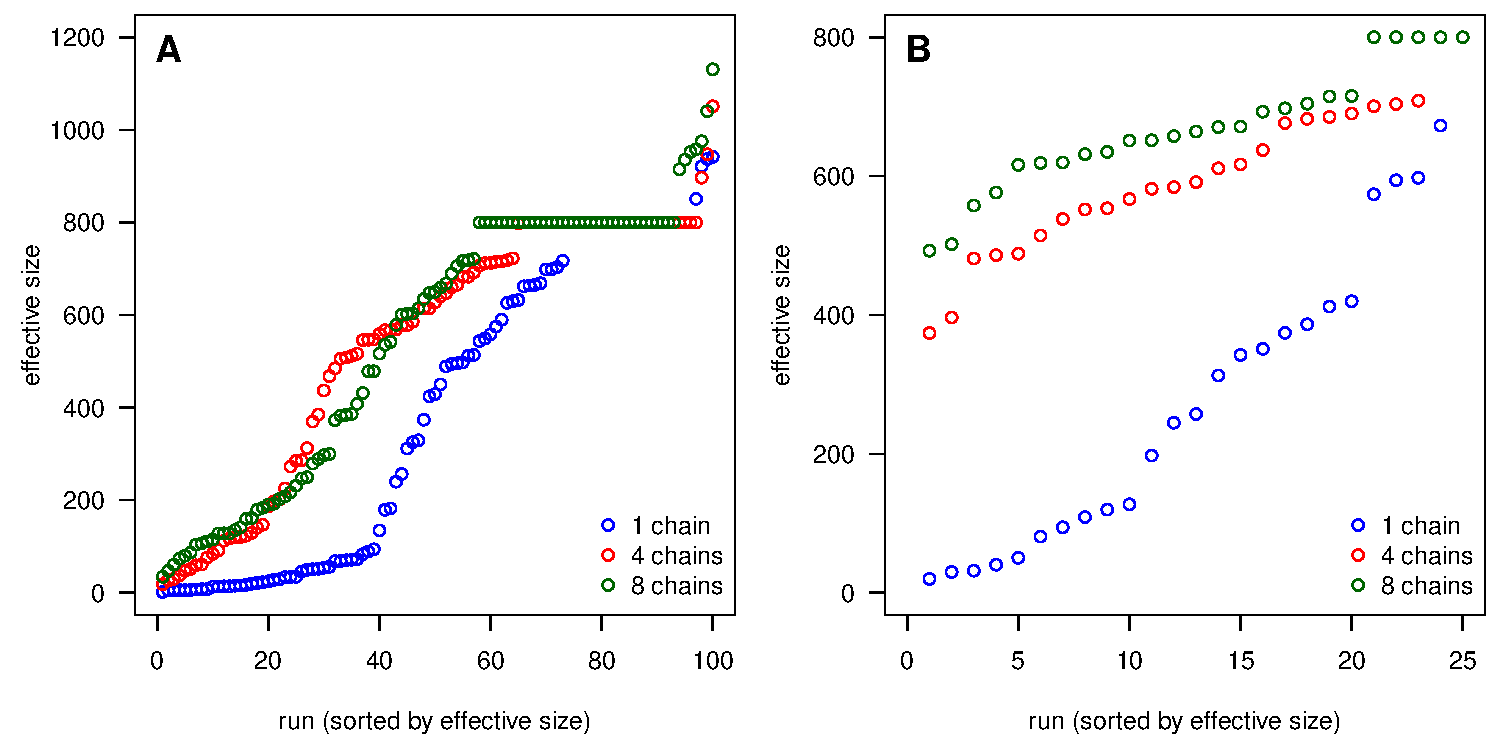
\includegraphics[width=14cm]{eff-size.pdf}
\end{center}
\caption{Effective sizes of the log-likelihood samples
    for runs with 1, 4, or 8 chains in
    (a) runs of 100 simulated trees and (b) 25 runs of the skink tree.
    Runs are sorted by their effective size,
    and higher effective size indicates better mixing.
    For both simulated trees and the skink tree,
    runs with 4 or 8 chains (Metropolis-coupled MCMC)
    had better mixing than runs with a single chain.}
\label{fig:eff-size}
\end{figure}


\subsection*{Convergence}

For the skink runs without \MCMCMC,
the lower and upper 5\% quantiles ($\times$ 1,000)
of the median log-likelihood variances were 9.80--20.69 (mean of 14.99).
%
For the treatments with four and eight chains,
the quantiles ($\times$ 1,000) were 4.71--10.53 (mean of 7.46)
and 4.32--10.70 (mean of 7.35).
%
These results indicate that the median log-likelihood variance
in runs without \MCMCMC\ were higher than those with \MCMCMC\ 
(with a small amount of overlap).
%
These result suggest that runs with \MCMCMC\ 
converged better than those without \MCMCMC.


\subsection*{Median log-likelihood}

We found that for the runs with simulated trees,
the median log-likelihood values among treatments
were virtually identical per replicate runs (Figure~\ref{fig:median-log-like}a).
%
These results indicate that for simulated trees,
the MCMC simulation found the same posterior probability distribution,
whether it had one, four, or eight chains.
%
For the skink tree runs,
the mean median log-likelihood (and 95\% bootstrap confidence interval)
with one chain was $-631.29$ ($-631.34$--$-631.25$),
with four chains it was $-631.16$ ($-631.19$--$-631.12$),
with eight chains it was $-631.12$ ($-631.15$--$-631.08$)
(Figure~\ref{fig:median-log-like}b).
%
These results indicate that the MCMC simulation
reached a higher log-likelihood space
(i.e., more probable shift configurations)
with \MCMCMC\ than without it.

\begin{figure}
\begin{center}
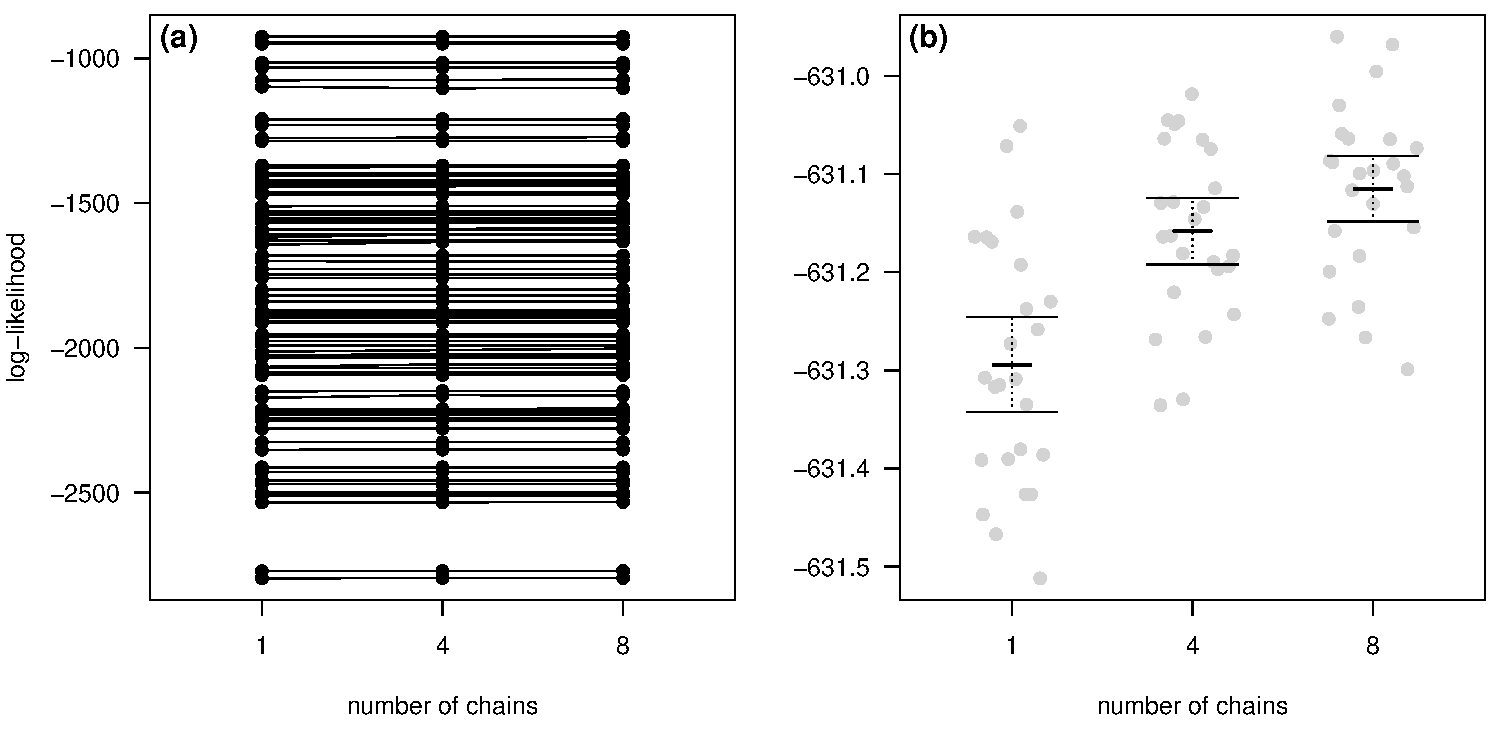
\includegraphics[width=14cm]{median-log-like.pdf}
\end{center}
\caption{Median log-likelihoods for (a) runs of 100 simulated trees
    and (b) 25 runs of the skink tree.
    Each solid circle represents the median log-likelihood of a single run.
    In (a), lines connect runs with the same simulated tree.
    In (b), the thick lines are the mean of the median log-likelihoods
    and the thin lines are the edges of the 95\% confidence intervals.
    The gray circles are jittered horizontally for clarity.
    For the simulated trees (a), the median log-likelihoods were the same
    across treatments.
    For the skink tree (b), the median log-likelihoods were greater
    with 4 or 8 chains than with a single chain.}
\label{fig:median-log-like}
\end{figure}


\subsection*{Speed}

We found that the parallellism of \MCMCMCMC\ 
reduced the amount of time runs would have taken without it.
%
For the simulated trees, which ran for 25 million generations,
the mean number of hours that runs took with
one chain, four chains, and eight chains were
6.3, 6.5, and 6.8 h.
%
Without \MCMCMCMC, the runs with four and eight chains
would have taken 25.2 and 50.4 h.
%
For the skink tree, which ran for 100 million generations,
the means were 18.8, 20.7, and 21.4 h for one, four, and eight chains.
%
Without \MCMCMCMC, the runs with four and eight chains
would have taken 75.2 h (3.1 d) and 150.5 h (6.3 d).


% Point out the importance of the results and place them in the context
% of previous studies and in relation to the application of the work
% (expanding on the Synthesis and applications section of the Summary).
% Where appropriate, set out recommendations for management or policy
\section*{Discussion}

We have found that Metropolis-coupled MCMC improves
the overall performance of BAMM analyses.
%
In order to unbiased results,
it is important that samples be indepentent.

% In Fig. 3, why does panel (a) results all start at 0,
% but for panel (b), MC3 results start way higher?
% - Look at simulated data to see why some have eff. size of 0

% In Fig. 4, why did simulations not improve log-likelihood with MC3,
% but they did for the skink tree?
% - Indicates simulations all reached the same place
% - Perhaps they got stuck there, maybe solution was simple
%   - Check to see whether they all found four events

% In Fig. 4, more chains seems to improve log-likelihood (8 vs. 4)
% - More chains can explore more landscape
% - But diminishing returns (1 vs. 4 vs. 8)


\section*{Acknowledgements}
This research was supported in part by
NSF-DEB-1256330 to DLR, and through computational resources
and services provided by Advanced Research Computing
at the University of Michigan, Ann Arbor.


\bibliography{mc3}

\end{document}
